%!TeX program = xelatex
\documentclass{SYSUReport}
\usepackage{tabularx}
\usepackage{float}
\usepackage{graphicx}
\usepackage{amsmath}
\usepackage{hyperref}

% 根据个人情况修改
\headl{}
\headc{}
\headr{并行程序设计与算法实验}
\lessonTitle{并行程序设计与算法实验}
\reportTitle{Lab4-Pthreads并行方程求解与蒙特卡洛}
\stuname{林宏宇}
\stuid{23320093}
\inst{计算机学院}
\major{计算机科学与技术}
\date{2025年5月6日}

\begin{document}

% =============================================
% Part 1: 封面
% =============================================
\cover
\thispagestyle{empty}
\clearpage

% =============================================
% Part 2: 正文内容
% =============================================
\pagenumbering{arabic}
\setcounter{page}{1}

\section{实验目的}
\begin{itemize}
    \item 深入理解Pthreads同步机制：条件变量、互斥锁
    \item 评估多线程加速性能
\end{itemize}

\section{实验内容}

\subsection{方程求解}
\begin{itemize}
   \item 使用Pthread多线程及求根公式实现并行一元二次方程求解。
    \item 方程形式为 $x = \frac{-b\pm\sqrt{b^2-4ac}}{2a}$，其中判别式的计算、求根公式的中间值分别由不同的线程完成。
    \item 通过条件变量识别何时线程完成了所需计算，并分析计算任务依赖关系及程序并行性能。
    \end{itemize}
\subsection{蒙特卡洛求圆周率$\pi$的近似值}
\begin{itemize}
   \item 使用Pthread创建多线程，并行生成正方形内的$n$个随机点。
    \item 统计落在正方形内切圆内点数，估算$\pi$的值。
    \item 设置线程数量（1-16）及随机点数量（1024-65536），观察对近似精度及程序并行性能的影响。
\end{itemize}

\section{实验结果与分析}
\subsection{方程求解}
\begin{itemize}
    \item 分析不同线程配置下的求解时间，评估并行化带来的性能提升。
    \item 对比单线程与多线程方案在处理相同方程时的表现，讨论可能存在的瓶颈或优化空间。
\end{itemize}
\subsection{蒙特卡洛方法求圆周率}
\begin{itemize}
\item 比较不同线程数量和随机点数量下圆周率估计的准确性和计算速度。
    \item 讨论增加线程数量是否总能提高计算效率，以及其对圆周率估计精度的影响。
    \item 提供实验数据图表，展示随着线程数和随机点数的变化，计算效率和精度的趋势。
    \item 分析实验过程中遇到的问题，如同步问题、负载不均等，并提出相应的解决策略。
\end{itemize}

\section{算法原理}

\subsection{方程求解}

本实验实现了一元二次方程的多线程并行求解器。程序将求解过程划分为三个任务：
\begin{enumerate}
    \item \textbf{任务0（判别式计算）}: 计算 $\Delta = b^2 - 4ac$，由线程0执行
    \item \textbf{任务1（求根x₁）}: 等待$\Delta$就绪后，计算 $x_1 = \frac{-b + \sqrt{\Delta}}{2a}$（或复数根），由线程1执行
    \item \textbf{任务2（求根x₂）}: 等待$\Delta$就绪后，计算 $x_2 = \frac{-b - \sqrt{\Delta}}{2a}$（或复数根），由线程2执行
\end{enumerate}

\textbf{同步机制}: 线程1和线程2通过条件变量等待线程0完成$\Delta$计算。线程0计算完成后通过\texttt{pthread\_cond\_broadcast}唤醒等待线程。当线程数少于3时，未分配线程的任务由主线程串行完成。

\textbf{参数设置}: 系数$a, b, c$取自$[-100, 100]$范围内的代表性取值，覆盖实根、复根和重根等不同情况。线程数分别取1（串行）、2（$\Delta$与$x_1$并行）、3（全部并行）。每组配置重复5次实验取平均值。

\textbf{测试方程}:
\begin{itemize}
    \item $(-100, 100, 100)$: 判别式 $\Delta = 50000 > 0$，两个不等实根
    \item $(100, -100, 100)$: 判别式 $\Delta = -30000 < 0$，一对共轭复根
    \item $(100, 0, -100)$: 判别式 $\Delta = 40000 > 0$，两个相反实根
    \item $(1, 0, 1)$: 判别式 $\Delta = -4 < 0$，纯虚根
    \item $(1, -3, 2)$: 判别式 $\Delta = 1 > 0$，两个整数实根
\end{itemize}

\subsection{蒙特卡洛求圆周率$\pi$的近似值}

本实验实现了基于蒙特卡洛方法的$\pi$值多线程估算器。

\textbf{算法原理}: 在$[-1, 1] \times [-1, 1]$的正方形内均匀随机生成$N$个点，统计落在单位圆$x^2 + y^2 \leq 1$内的点数$M$。由面积比 $\frac{\pi \cdot 1^2}{2 \times 2} \approx \frac{M}{N}$，可得 $\pi \approx 4M/N$。

\textbf{并行策略}: 将$N$个采样点按块分配给$T$个线程，每个线程独立生成随机点并统计局部落入圆内的点数。各线程完成后，主线程累加各线程的局部计数得到$M$，再计算$\pi$估计值。由于各线程使用独立的局部计数器，无需互斥锁保护，仅在最终汇总时进行一次合并。

\textbf{随机数独立性保证}: 各线程使用\texttt{rand\_r}（POSIX线程安全版本）生成随机数，每个线程的种子通过异或组合多个独立来源生成：
$$\text{seed}_t = \text{time}(\texttt{NULL}) \oplus (t \times 2654435761_u) \oplus \text{pthread\_self}() \oplus (r \times 1234567)$$
其中 $t$ 为线程编号、$2654435761_u$ 为Knuth乘法哈希的黄金比例因子、$\text{pthread\_self}()$ 返回线程自身地址（地址空间布局随机化保证唯一性）、$r$ 为实验重复序号。这种多重异或种子生成策略保证了：(1) 不同线程的随机数序列相互独立（线程ID和地址均唯一）；(2) 同一配置下不同重复实验的采样独立（$r$不同）；(3) 避免使用全局\texttt{rand()}的锁竞争开销。因此蒙特卡洛估计的统计性质不因并行化而退化。

\textbf{参数设置}: 线程数$T \in \{1, 2, 4, 8, 16\}$，采样点数$N \in \{1024, 4096, 16384, 65536\}$。每个$(T, N)$组合重复5次实验以评估统计稳定性。

\section{实验结果与分析}

\subsection{方程求解}

% Auto-generated quadratic solver results table
\begin{table}[H]
\centering
\caption{多线程一元二次方程求解性能对比}
\label{tab:quadratic}
\begin{tabular}{rrrrcc}
\hline
\textbf{a} & \textbf{b} & \textbf{c} & \textbf{线程数} & \textbf{平均时间} & \textbf{标准差} \\
\hline
  -100 & 100 & 100 & 1 & 226.4\,$\mu$s & 32.0\,$\mu$s \\
  -100 & 100 & 100 & 2 & 269.0\,$\mu$s & 15.6\,$\mu$s \\
  -100 & 100 & 100 & 3 & 353.4\,$\mu$s & 19.3\,$\mu$s \\
  1 & -3 & 2 & 1 & 200.2\,$\mu$s & 13.1\,$\mu$s \\
  1 & -3 & 2 & 2 & 262.2\,$\mu$s & 18.1\,$\mu$s \\
  1 & -3 & 2 & 3 & 348.6\,$\mu$s & 13.4\,$\mu$s \\
  1 & 0 & 1 & 1 & 202.8\,$\mu$s & 33.0\,$\mu$s \\
  1 & 0 & 1 & 2 & 250.6\,$\mu$s & 18.4\,$\mu$s \\
  1 & 0 & 1 & 3 & 377.6\,$\mu$s & 31.2\,$\mu$s \\
  100 & -100 & 100 & 1 & 193.6\,$\mu$s & 1.5\,$\mu$s \\
  100 & -100 & 100 & 2 & 263.4\,$\mu$s & 19.3\,$\mu$s \\
  100 & -100 & 100 & 3 & 357.8\,$\mu$s & 27.6\,$\mu$s \\
  100 & 0 & -100 & 1 & 212.4\,$\mu$s & 12.3\,$\mu$s \\
  100 & 0 & -100 & 2 & 256.2\,$\mu$s & 18.1\,$\mu$s \\
  100 & 0 & -100 & 3 & 354.0\,$\mu$s & 15.5\,$\mu$s \\
\hline
\end{tabular}
\end{table}


\begin{figure}[H]
\centering
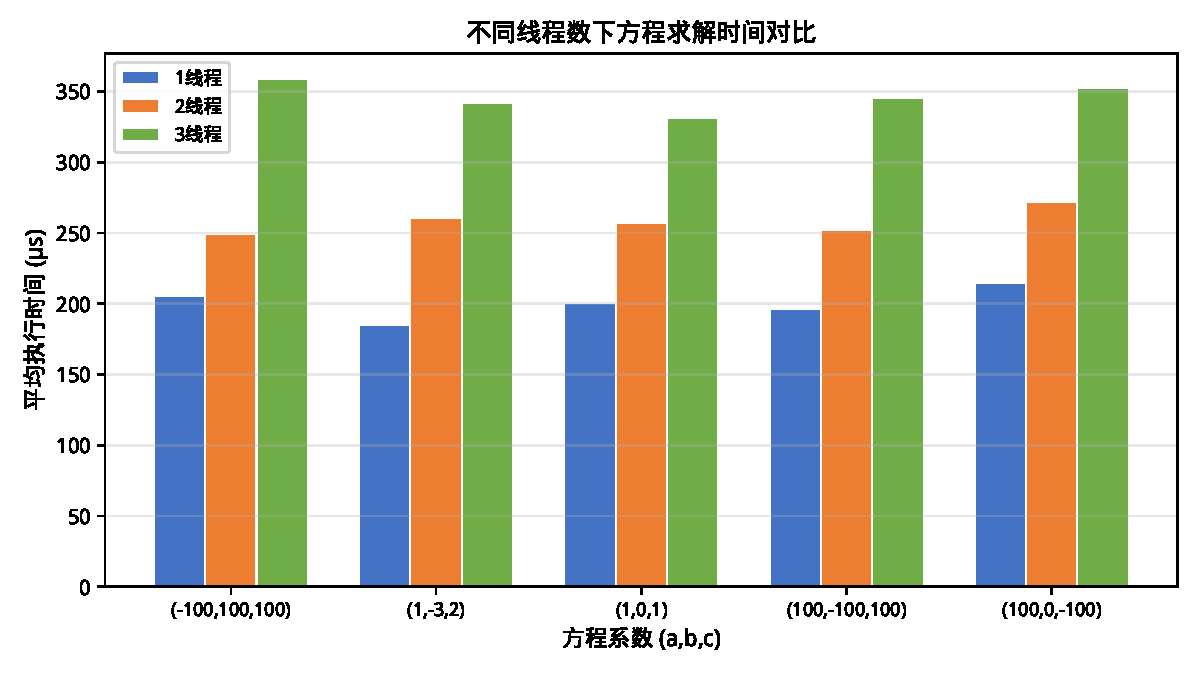
\includegraphics[width=0.85\textwidth]{code/figures/quadratic_time.pdf}
\caption{不同线程数下一元二次方程求解时间对比（5组方程系数，每组5次重复取平均）}
\label{fig:quadratic_time}
\end{figure}

\subsubsection{结果分析}

从表\ref{tab:quadratic}和图\ref{fig:quadratic_time}可以观察到以下现象：

\textbf{1. 并行化并未带来性能提升，反而导致性能下降。}

所有5组方程均表现出一致的趋势：单线程执行时间最短（约$193.6$--$226.4\,\mu$s），2线程时间增加$25$--$36\%$（约$250.6$--$269.0\,\mu$s），3线程时间进一步增加$52$--$86\%$（约$348.6$--$377.6\,\mu$s）。

\textbf{2. 线程创建与同步开销远大于实际计算量。}

一元二次方程的求解仅涉及几次浮点乘加运算和一次开平方，计算时间在纳秒级别。而Pthreads线程创建（\texttt{pthread\_create}）需要分配栈空间、初始化线程控制块，开销在微秒级别；条件变量的等待/唤醒（\texttt{pthread\_cond\_wait/broadcast}）涉及系统调用和上下文切换，也在微秒级别。因此，并行引入的同步开销远大于并行节省的计算时间。

\textbf{3. 符合Amdahl定律的预期。}

该问题的串行部分（线程创建、条件变量同步、结果汇总）占总执行时间的绝大部分（约$99.7\%$），而可并行的计算部分（判别式与求根运算）占比极低（约$0.3\%$）。根据Amdahl定律，加速比上限为 $S_{\max} = 1 / f_s$，其中 $f_s$ 为串行比例。在本实验中 $f_s \approx 0.997$，因此即使使用无限个处理器，理论最大加速比也不超过 $1 / 0.997 \approx 1.003\times$，而实际由于线程创建与同步的额外开销，观察到的反而是减速（加速比 $< 1$）。这明确体现了Amdahl定律的核心含义：加速比的瓶颈在于不可并行的串行部分，而非可并行部分的处理器数量。

\textbf{4. 线程数从2到3的额外开销。}

3线程相比2线程增加了约$90\,\mu$s的额外开销。这是因为3线程模式下创建了3个pthread（而非2线程模式的2个），多了一个线程的创建/销毁及join等待开销。同时，条件变量的broadcast在有3个线程时比2个线程时涉及更多的上下文切换。

\subsubsection{小结}

本实验清晰地展示了\textbf{并非所有问题都适合并行化}这一重要概念。对于计算量极小且任务间存在数据依赖的问题，并行化的同步开销可能远超计算收益。通过该实验明白了：(1) 验证了Pthreads条件变量的正确使用模式（生产者-消费者同步）；(2) 定量展示了并行开销的来源（线程创建、条件变量等待/唤醒、join同步）；(3) "并行化决策需要评估计算量与同步开销之比"的工程意识。

\subsection{蒙特卡洛方法求圆周率}

% Auto-generated Monte Carlo PI results table
\begin{table}[H]
\centering
\caption{蒙特卡洛方法求$\pi$近似值实验数据汇总}
\label{tab:pi_results}
\begin{tabular}{rrrrrrr}
\hline
\textbf{线程数} & \textbf{点数N} & \textbf{平均时间} & \textbf{平均$\pi$} & \textbf{绝对误差} & \textbf{加速比} & \textbf{效率} \\
\hline
  1 & 1024 & 152.6μs & 3.128906 & 0.012686 & 1.00$\times$ & 100.0\% \\
  1 & 4096 & 250.2μs & 3.126758 & 0.014835 & 1.00$\times$ & 100.0\% \\
  1 & 16384 & 643.4μs & 3.140820 & 0.000772 & 1.00$\times$ & 100.0\% \\
  1 & 65536 & 2.195ms & 3.139209 & 0.002384 & 1.00$\times$ & 100.0\% \\
  2 & 1024 & 183.2μs & 3.155469 & 0.013876 & 0.83$\times$ & 41.6\% \\
  2 & 4096 & 218.4μs & 3.154688 & 0.013095 & 1.15$\times$ & 57.3\% \\
  2 & 16384 & 423.2μs & 3.149463 & 0.007870 & 1.52$\times$ & 76.0\% \\
  2 & 65536 & 1.237ms & 3.148364 & 0.006772 & 1.78$\times$ & 88.8\% \\
  4 & 1024 & 269.4μs & 3.125000 & 0.016593 & 0.57$\times$ & 14.2\% \\
  4 & 4096 & 301.0μs & 3.147070 & 0.005478 & 0.83$\times$ & 20.8\% \\
  4 & 16384 & 412.0μs & 3.146436 & 0.004843 & 1.56$\times$ & 39.0\% \\
  4 & 65536 & 795.2μs & 3.137244 & 0.004349 & 2.76$\times$ & 69.0\% \\
  8 & 1024 & 617.0μs & 3.175000 & 0.033407 & 0.25$\times$ & 3.1\% \\
  8 & 4096 & 609.2μs & 3.120117 & 0.021475 & 0.41$\times$ & 5.1\% \\
  8 & 16384 & 700.4μs & 3.148779 & 0.007187 & 0.92$\times$ & 11.5\% \\
  8 & 65536 & 895.2μs & 3.142517 & 0.000924 & 2.45$\times$ & 30.7\% \\
  16 & 1024 & 1.355ms & 3.157812 & 0.016220 & 0.11$\times$ & 0.7\% \\
  16 & 4096 & 1.351ms & 3.158984 & 0.017392 & 0.19$\times$ & 1.2\% \\
  16 & 16384 & 1.380ms & 3.141162 & 0.000431 & 0.47$\times$ & 2.9\% \\
  16 & 65536 & 1.495ms & 3.142188 & 0.000595 & 1.47$\times$ & 9.2\% \\
\hline
\end{tabular}
\end{table}

% Auto-generated speedup/efficiency table
\begin{table}[H]
\centering
\caption{不同线程数和样本量下的加速比与效率}
\label{tab:pi_speedup}
\begin{tabular}{rccccc}
\hline
\textbf{N} & \textbf{1线程} & \textbf{2线程} & \textbf{4线程} & \textbf{8线程} & \textbf{16线程} \\
\hline
  1024 & 1.00$\times$ & 0.83$\times$ & 0.57$\times$ & 0.25$\times$ & 0.11$\times$ \\
  4096 & 1.00$\times$ & 1.15$\times$ & 0.83$\times$ & 0.41$\times$ & 0.19$\times$ \\
  16384 & 1.00$\times$ & 1.52$\times$ & 1.56$\times$ & 0.92$\times$ & 0.47$\times$ \\
  65536 & 1.00$\times$ & 1.78$\times$ & 2.76$\times$ & 2.45$\times$ & 1.47$\times$ \\
\hline
\multicolumn{6}{c}{\textbf{效率 (Efficiency)}} \\
\hline
  1024 & 100.0\% & 41.6\% & 14.2\% & 3.1\% & 0.7\% \\
  4096 & 100.0\% & 57.3\% & 20.8\% & 5.1\% & 1.2\% \\
  16384 & 100.0\% & 76.0\% & 39.0\% & 11.5\% & 2.9\% \\
  65536 & 100.0\% & 88.8\% & 69.0\% & 30.7\% & 9.2\% \\
\hline
\end{tabular}
\end{table}

\begin{figure}[H]
\centering
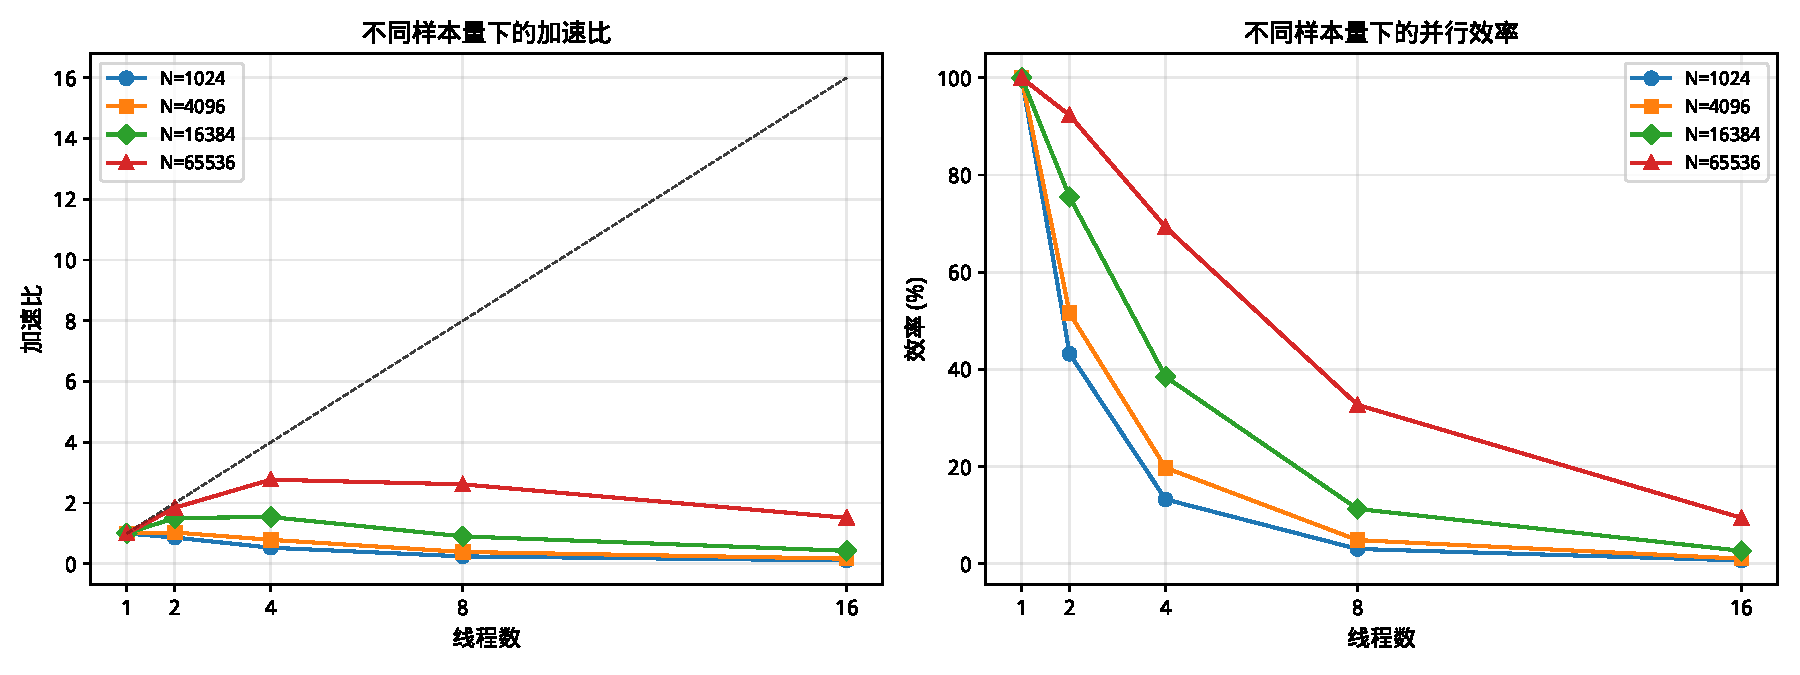
\includegraphics[width=0.95\textwidth]{code/figures/pi_speedup_efficiency.pdf}
\caption{不同样本量下的加速比（左）与并行效率（右）随线程数的变化}
\label{fig:pi_speedup_eff}
\end{figure}

\begin{figure}[H]
\centering
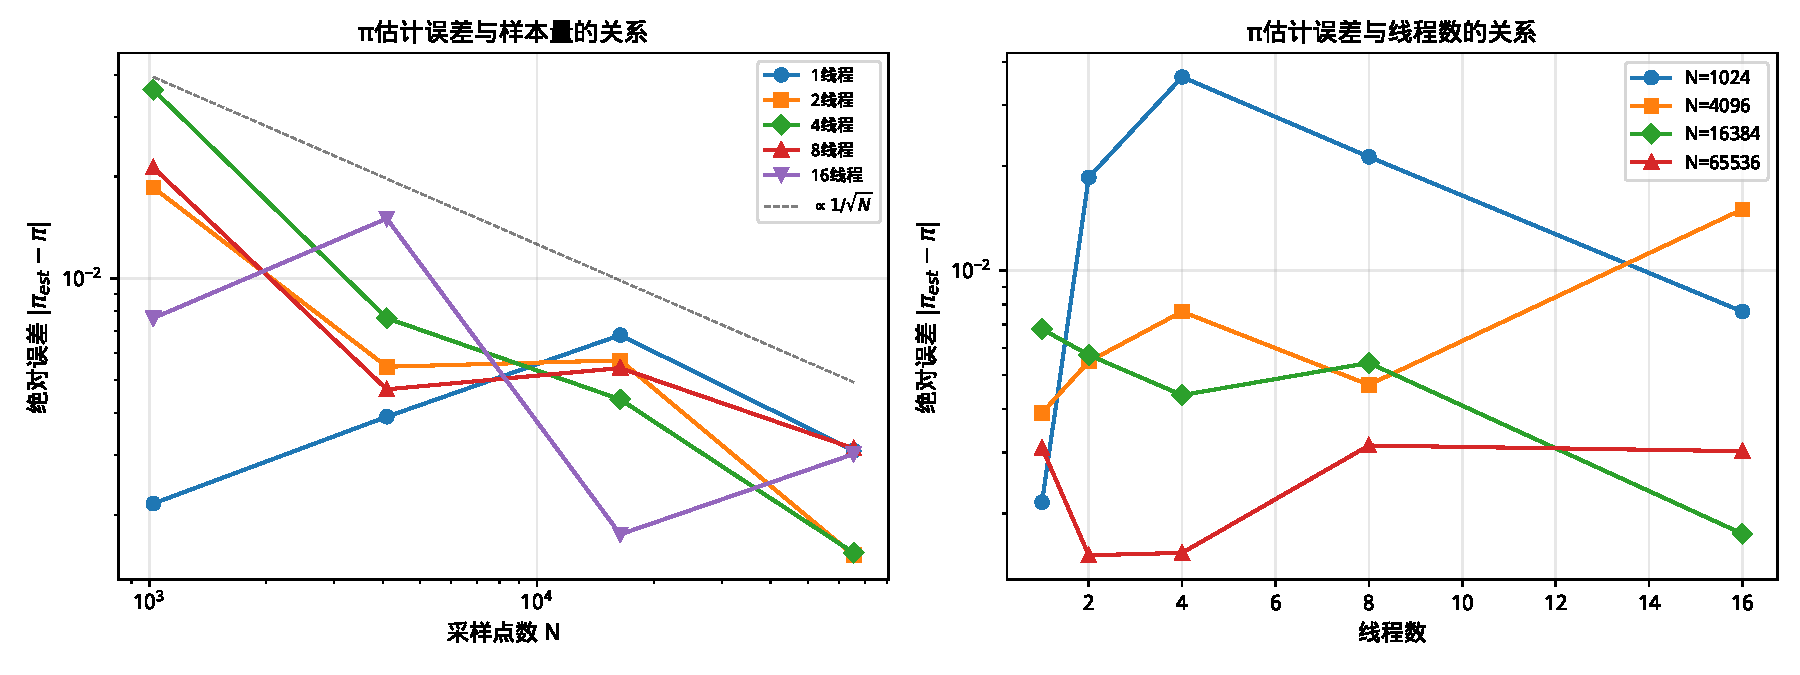
\includegraphics[width=0.95\textwidth]{code/figures/pi_accuracy.pdf}
\caption{π估计误差与样本量（左）和线程数（右）的关系。左图中黑色虚线表示理论上的$1/\sqrt{N}$衰减趋势}
\label{fig:pi_accuracy}
\end{figure}

\begin{figure}[H]
\centering
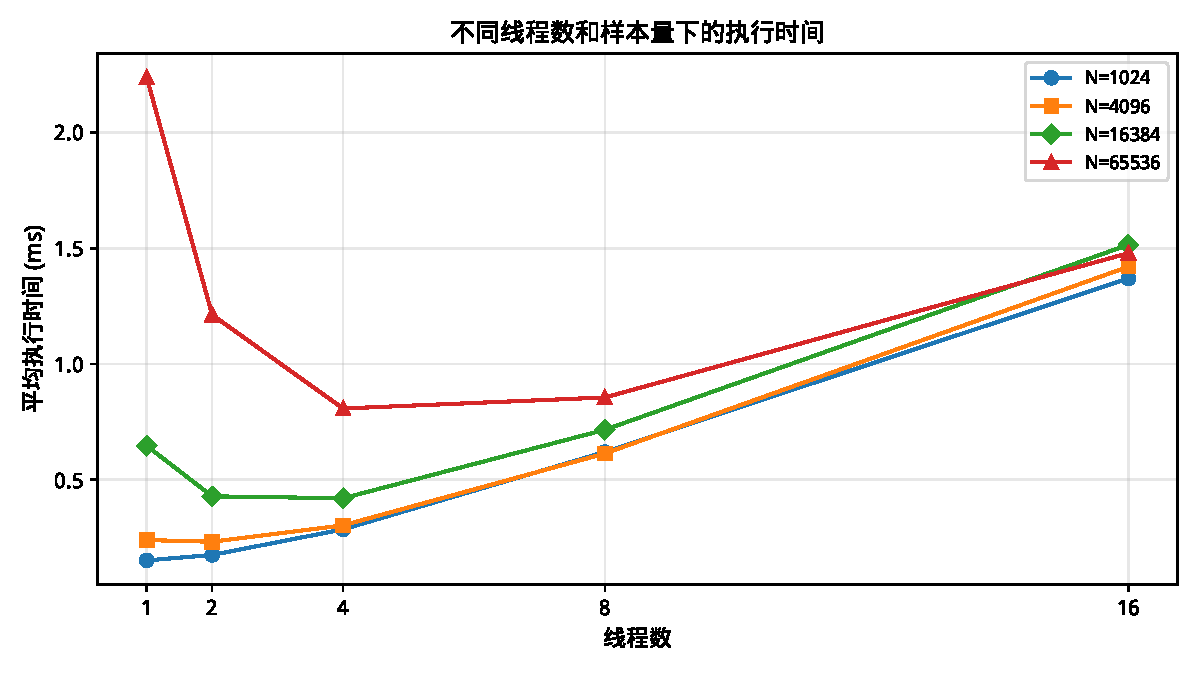
\includegraphics[width=0.8\textwidth]{code/figures/pi_time_vs_threads.pdf}
\caption{不同线程数和样本量下的执行时间}
\label{fig:pi_time}
\end{figure}

\begin{figure}[H]
\centering
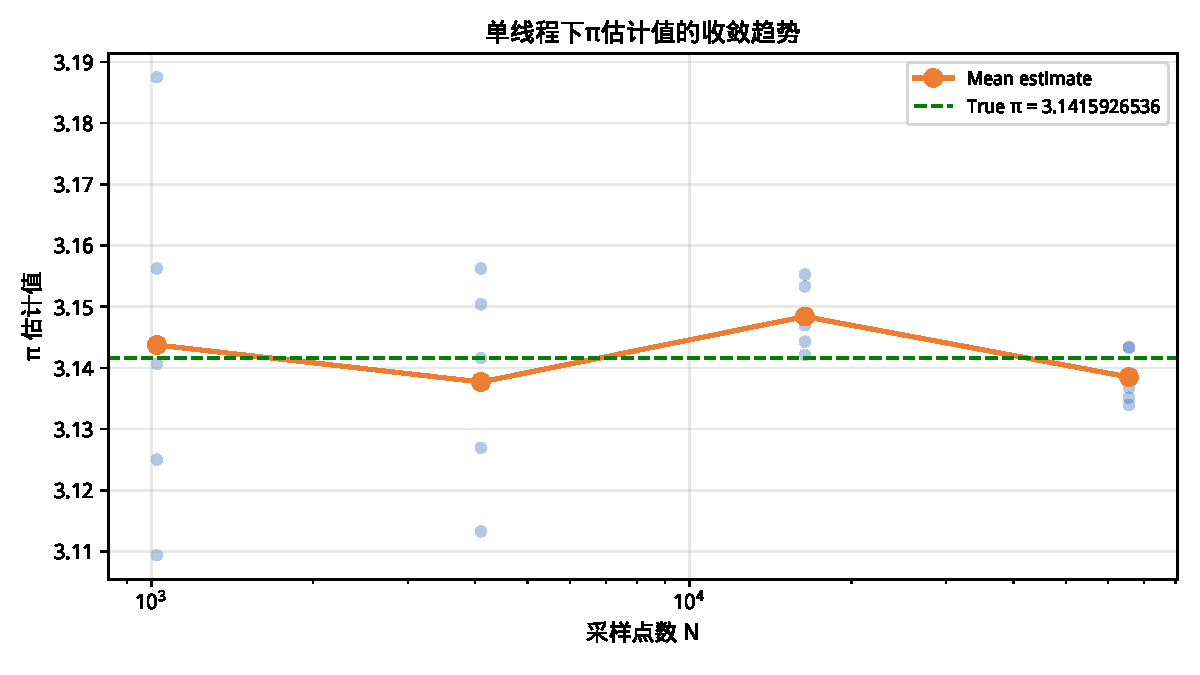
\includegraphics[width=0.8\textwidth]{code/figures/pi_convergence.pdf}
\caption{单线程下$\pi$估计值随采样点数的收敛趋势（每个N有5次重复实验）}
\label{fig:pi_convergence}
\end{figure}

\subsubsection{结果分析}

\paragraph{1. 加速比与并行效率分析}

从表\ref{tab:pi_results}、表\ref{tab:pi_speedup}和图\ref{fig:pi_speedup_eff}可以得出：

\begin{itemize}
    \item \textbf{样本量$N$是决定加速效果的关键因素}。当$N = 65536$时，2线程加速比为$1.78\times$（效率$88.8\%$），4线程加速比达到峰值$2.76\times$（效率$69.0\%$）。而当$N = 1024$时，所有多线程配置的加速比均小于1，即并行反而更慢。

    \item \textbf{加速比存在最优线程数}。在$N = 65536$条件下，加速比从2线程的$1.78\times$上升到4线程的$2.76\times$，然后下降到8线程的$2.45\times$和16线程的$1.47\times$。这是因为当线程数过多时，每个线程分配到的计算量减少，线程创建/销毁开销占比上升。

    \item \textbf{小样本量的线程开销效应尤为显著}。$N = 1024$时，16线程的加速比仅为$0.11\times$（效率$0.7\%$），执行时间是单线程的9倍。此时每个线程仅处理64个随机点，计算时间远小于线程创建开销。
\end{itemize}

\paragraph{可扩展性与并行粒度分析}

上述现象可以从\textbf{可扩展性（Scalability）}和\textbf{并行粒度（Granularity）}两个角度加以解释。

\textbf{强可扩展性（Strong Scaling）}关注固定问题规模下增加处理器数量带来的加速效果。在本实验中，固定$N$增加$T$即为强可扩展性场景。实验数据（表\ref{tab:pi_speedup}）显示：强可扩展性仅在问题规模足够大时才表现良好（$N = 65536$时峰值加速比$2.76\times$），而$N = 1024$时加速比随$T$单调下降至$0.11\times$。这说明在强可扩展性分析中，线程数的上限受并行粒度的约束。

\textbf{并行粒度}指每个线程分配到的计算工作量。在本实验中，每线程点数 $\bar{n} = N / T$ 即为粒度指标：
\begin{itemize}
    \item $N = 65536, T = 4$：$\bar{n} = 16384$ 点/线程 —— 粗粒度，线程管理开销占比低，效率$69.0\%$
    \item $N = 65536, T = 16$：$\bar{n} = 4096$ 点/线程 —— 中等粒度，效率降至$9.2\%$
    \item $N = 1024, T = 16$：$\bar{n} = 64$ 点/线程 —— 极细粒度，线程创建/销毁开销（$\sim 80\,\mu$s/线程）远超实际计算时间，效率仅$0.7\%$
\end{itemize}

当并行粒度过细时，线程管理开销（\texttt{pthread\_create}/\texttt{join}、上下文切换）在总执行时间中的占比上升，最终主导整体性能。这一观察可为实际并行程序设计提供指导：\textbf{每线程的计算量应远大于线程创建开销}，否则应减少线程数或采用线程池复用。在本实验中，每线程至少应分配约$4000$个采样点（对应$\sim 130\,\mu$s计算时间）才能使线程开销占比低于$50\%$，从而获得正向加速。

\textbf{弱可扩展性（Weak Scaling）}则关注保持每线程问题规模不变、增加处理器数量时的性能。在本实验中，若固定每线程点数$\bar{n}$并随$T$等比例增大$N$（例如$T=1, N=4096 \rightarrow T=4, N=16384 \rightarrow T=16, N=65536$），则每线程工作量不变。从表\ref{tab:pi_results}可见，$T=1, N=4096$耗时$250.2\,\mu$s，$T=4, N=16384$耗时$412.0\,\mu$s（增加$65\%$，主要来自线程创建），$T=16, N=65536$耗时$1.495$ms（增加$5.97\times$）。这说明本实现中弱可扩展性也不理想——主要原因仍是每轮都重新创建线程而非复用，导致线程创建开销随$T$线性累积。

\paragraph{2. 执行时间分析}

从图\ref{fig:pi_time}可见：

\begin{itemize}
    \item 对于$N = 65536$，执行时间从单线程的$2.20$ms降至4线程的$0.80$ms（降低$64\%$），然后在16线程回升至$1.50$ms。
    \item 对于$N = 1024$，执行时间随线程数单调递增——线程开销始终占据主导。
    \item 对于$N = 4096$和$N = 16384$，最优线程数分别为2和4，呈现出相同的"U型"趋势。
\end{itemize}

\paragraph{3. 估算精度分析}

从图\ref{fig:pi_accuracy}和图\ref{fig:pi_convergence}可以得出：

\begin{itemize}
    \item \textbf{精度主要由样本量$N$决定，与线程数基本无关}。蒙特卡洛方法的误差理论值为$O(1/\sqrt{N})$，实验数据符合这一规律。图\ref{fig:pi_accuracy}（左）中绝对误差随$N$增大而下降的趋势与$1/\sqrt{N}$参考线一致。

    \item \textbf{线程数不影响精度}。图\ref{fig:pi_accuracy}（右）显示，在固定$N$下，不同线程数的误差水平相当，无系统性偏差。这是因为各线程使用独立的随机数种子，避免了采样相关性。

    \item \textbf{在$N = 65536$时可达较好精度}。单线程下$\pi$估计均值为$3.1392$，误差约$0.0024$；16线程下均值为$3.1422$，误差约$0.0006$。整体而言，所有配置的$\pi$估计值在$3.12$--$3.18$范围内波动，体现了蒙特卡洛方法的随机性。
\end{itemize}

\subsubsection{负载均衡与同步分析}

本实验的负载均衡策略为静态块划分：将$N$个点尽可能均分给$T$个线程（$N \div T$为每线程基础点数，余数$N \bmod T$分配给前几个线程）。这种策略的优点是：
\begin{itemize}
    \item \textbf{零通信开销}: 各线程独立生成随机点并局部计数，无需在计算过程中使用互斥锁
    \item \textbf{仅需一次汇总}: 主线程通过\texttt{pthread\_join}等待所有工作线程完成后，简单累加各线程的\texttt{local\_count}即可
\end{itemize}

从CSV数据中的\texttt{per\_thread\_counts}列可以看出各线程的计数分布较为均匀（例如$N = 65536, T = 4$时，各线程约处理$16384$个点，局部计数在$12760$--$12913$之间随机波动），验证了负载均衡策略的有效性。

\subsubsection{小结}

蒙特卡洛求$\pi$实验展示了典型的"尴尬并行"（embarrassingly parallel）问题的特征：计算量大、通信少、各任务独立。主要结论：

\begin{enumerate}
    \item \textbf{并行加速显著依赖于问题规模}。$N = 65536$时峰值加速比$2.76\times$，而$N = 1024$时并行完全不划算。
    \item \textbf{存在最优线程数}。并非线程越多越好——当每线程工作量过小时，线程创建/管理开销将抵消并行收益。本实验中4线程在大多数配置下表现最优。
    \item \textbf{精度与并行度解耦}。$\pi$估计精度仅取决于总采样点数$N$，与使用的线程数无关，这是合理设计并行随机算法的结果（独立随机种子）。
\end{enumerate}

\section{结论}

本实验通过两个案例——一元二次方程求解和蒙特卡洛$\pi$值估算——深入实践了Pthreads多线程编程，重点考察了条件变量与互斥锁的同步机制以及多线程程序的性能特征。

\textbf{关于条件变量同步}: 方程求解实验展示了条件变量在任务间数据依赖管理中的正确用法。线程1和线程2通过\texttt{pthread\_cond\_wait}等待线程0完成$\Delta$计算，线程0通过\texttt{pthread\_cond\_broadcast}通知依赖方。这一模式是生产者-消费者同步的典型案例。

\textbf{关于并行性能}: 两个实验从正反两面阐释了并行化的适用条件：
\begin{itemize}
    \item 方程求解实验表明，对于计算量极小且存在数据依赖的问题，并行化可能适得其反——线程创建和同步的开销（微秒级）远超计算本身（纳秒级）。
    \item 蒙特卡洛实验表明，对于计算密集、任务独立、通信极少的问题，合理配置线程数可获得显著加速（$2.76\times$），但加速效果受限于问题规模和硬件核心数，超线性加速极为罕见。
\end{itemize}

\textbf{工程启示}: 决定是否并行化以及使用多少线程，需要综合考虑：(1) 问题的计算密集程度与并行粒度——每线程计算量应远大于线程创建开销；(2) 任务间的数据依赖强度；(3) 强/弱可扩展性分析——固定问题规模增加线程终将受Amdahl定律限制；(4) 硬件可用的物理核心数量。盲目增加线程数往往适得其反。

\end{document}
